%----------------------------------------------------------------------------------------
%	PACKAGES AND OTHER DOCUMENT CONFIGURATIONS
%----------------------------------------------------------------------------------------

\documentclass{article}

\usepackage{fancyhdr} % Required for custom headers
\usepackage{lastpage} % Required to determine the last page for the footer
\usepackage{extramarks} % Required for headers and footers
\usepackage{graphicx} % Required to insert images
\usepackage{pdflscape} % Allow us to make certain pages in landscape orientation
\usepackage{amsmath} % Allow multiple line equations
\usepackage{amssymb}
\usepackage{scrextend}
\usepackage{xcolor}
\usepackage{listings}

\definecolor{mGreen}{rgb}{0,0.6,0}
\definecolor{mGray}{rgb}{0.5,0.5,0.5}
\definecolor{mPurple}{rgb}{0.58,0,0.82}
\definecolor{backgroundColour}{rgb}{0.95,0.95,0.92}

\lstdefinestyle{CStyle}{
    backgroundcolor=\color{backgroundColour},   
    commentstyle=\color{mGreen},
    keywordstyle=\color{magenta},
    numberstyle=\tiny\color{mGray},
    stringstyle=\color{mPurple},
    basicstyle=\footnotesize,
    breakatwhitespace=false,         
    breaklines=true,                 
    captionpos=b,                    
    keepspaces=true,                 
    numbers=none,                   
    numbersep=5pt,                  
    showspaces=false,                
    showstringspaces=false,
    showtabs=false,                  
    tabsize=2,
    language=C
}

% Margins
\topmargin=-0.45in
\evensidemargin=0in
\oddsidemargin=0in
\textwidth=6.5in
\textheight=9.0in
\headsep=0.25in 

\linespread{1.1} % Line spacing

% Set up the header and footer
\pagestyle{fancy}
\chead{\Title} % Top center header
\rhead{\firstxmark} % Top right header
\lfoot{\lastxmark} % Bottom left footer
\cfoot{} % Bottom center footer
\rfoot{Page\ \thepage\ of\ \pageref{LastPage}} % Bottom right footer
\renewcommand\headrulewidth{0.4pt} % Size of the header rule
\renewcommand\footrulewidth{0.4pt} % Size of the footer rule

\setlength\parindent{0pt} % Removes all indentation from paragraphs

%----------------------------------------------------------------------------------------
%	DOCUMENT STRUCTURE COMMANDS
%----------------------------------------------------------------------------------------

\setcounter{secnumdepth}{0} % Removes default section numbers
   
%----------------------------------------------------------------------------------------
%	NAME AND CLASS SECTION
%----------------------------------------------------------------------------------------

\newcommand{\Title}{Assignment 1} % Assignment title
\newcommand{\DueDate}{21 April 2018} % Due date
\newcommand{\Class}{CAB202 - Microprocessors and Digital Systems} % Course/class
\newcommand{\AuthorName}{Pedro Alves (n9424342)}

%----------------------------------------------------------------------------------------
%	TITLE PAGE
%----------------------------------------------------------------------------------------

\title{
\vspace{2in}
\textmd{\huge\textbf{\Class}}\\
\textmd{{\Title}}\\
\vspace{3in}
\textmd{{\AuthorName}}\\
}

%----------------------------------------------------------------------------------------

\begin{document}

\maketitle
\clearpage

%----------------------------------------------------------------------------------------
%	TABLE OF CONTENTS
%----------------------------------------------------------------------------------------

%\setcounter{tocdepth}{1} % Uncomment this line if you don't want subsections listed in the ToC

\newpage
\tableofcontents
\newpage

%----------------------------------------------------------------------------------------
%	EXECUTIVE SUMMARY
%----------------------------------------------------------------------------------------
\section{Executive Summary}

\clearpage

%----------------------------------------------------------------------------------------
%	PROGRAM OVERVIEW
%----------------------------------------------------------------------------------------
\section{Program Overview}
Things to talk about
\newline
change\_state
\clearpage

%----------------------------------------------------------------------------------------
%	SPLASH SCREEN
%----------------------------------------------------------------------------------------
\section{Splash Screen}
 The splash screen is the first screen the player sees when they start the game. It provides basic information about the game and will change to the main game screen when the player presses any key.

\subsection*{Functions}
\begin{lstlisting}[style=CStyle]
	// main.c
	void update_start_screen();
\end{lstlisting}
Called every tick of the main game loop. Will change the game's state to \emph{GAME\_SCREEN} if there is any key in the input buffer. Since the \emph{change\_state()} function already purges the input buffer, we do not have to worry about the game skipping straight to the \emph{GAME\_SCREEN}.
\begin{lstlisting}[style=CStyle]
	// main.c
	void draw_start_screen();
\end{lstlisting}
Calculates the x and y coordinates of each string to be shown based on the dimensions of the screen. Will then call \emph{draw\_string()} and \emph{draw\_center\_text()} multiple times to add the strings to the desired location.
\begin{lstlisting}[style=CStyle]
	// main.c
	void draw_center_text(char * text, int y);
\end{lstlisting}
Calculates what x coordinate is required in order to have the text appear at the middle of the screen. Then calls \emph{draw\_string()} to print the text. 
\newline

\subsection*{Testing}
Testing that the splash screen shows up when the game is started.
\begin{figure}[h]
	\begin{center}
	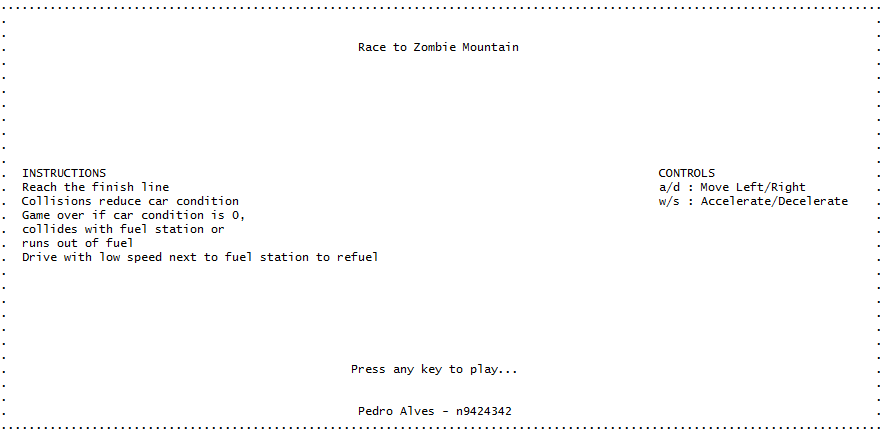
\includegraphics[width=1\textwidth]{images/splash_screen}
	\caption{The splash screen when the player starts the game}
	\label{fig:splash_screen} 
	\end{center}
\end{figure}

\clearpage

%----------------------------------------------------------------------------------------
%	BORDER
%----------------------------------------------------------------------------------------
\section{Border}
The border is simply a rectangle that is drawn on the edge of the terminal. It supports every terminal size.
\newline
The \emph{draw\_borders()} functon is the last one called before \emph{show\_screen()} in the draw step of the game loop. This ensures that no other graphics ever block the border. 

\subsection*{Globals}
\begin{lstlisting}[style=CStyle]
	// zombiemountain.h
	#define BORDER_CHAR	46
\end{lstlisting}
The character that will be used to represent the border. The number 46 represents the ASCII character "." (full stop).
\newline

\subsection*{Functions}
\begin{lstlisting}[style=CStyle]
	// main.c
	void draw_borders();
\end{lstlisting}
Draws 4 lines that form a rectangle on the edge of the screen. The length of these lines are calculated by using the screen width and height in order to make the borders work on every screen size.
\newline

\subsection*{Testing}
The game is started in different sized terminals and the borders are verified to have been drawn correctly.
\subsubsection*{Screen: 80x24}
\begin{figure}[h]
	\begin{center}
	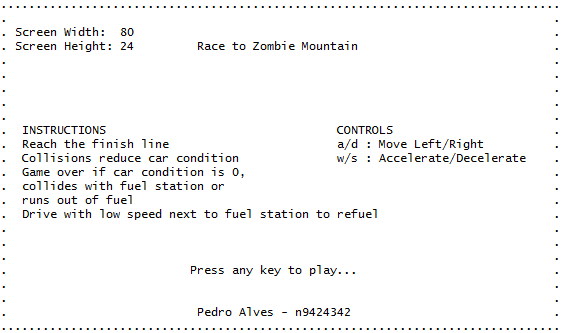
\includegraphics[width=0.95\textwidth]{images/border_80x24}
	\caption{The border with screen dimensions of 80x24}
	\label{fig:border_80x24} 
	\end{center}
\end{figure}
\subsubsection*{Screen: 126x31}
\begin{figure}[h]
	\begin{center}
	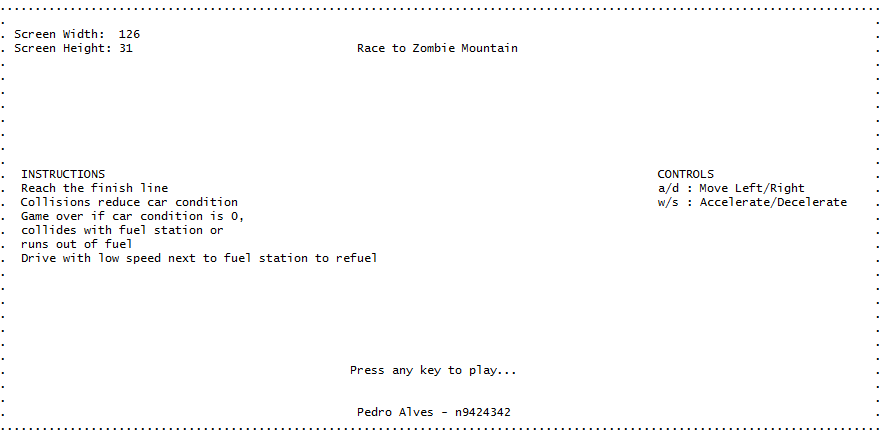
\includegraphics[width=1\textwidth]{images/border_126x31}
	\caption{The border with screen dimensions of 126x31}
	\label{fig:border_126x31} 
	\end{center}
\end{figure}
\subsubsection*{Screen: 190x50}
\begin{figure}[!ht]
	\begin{center}
	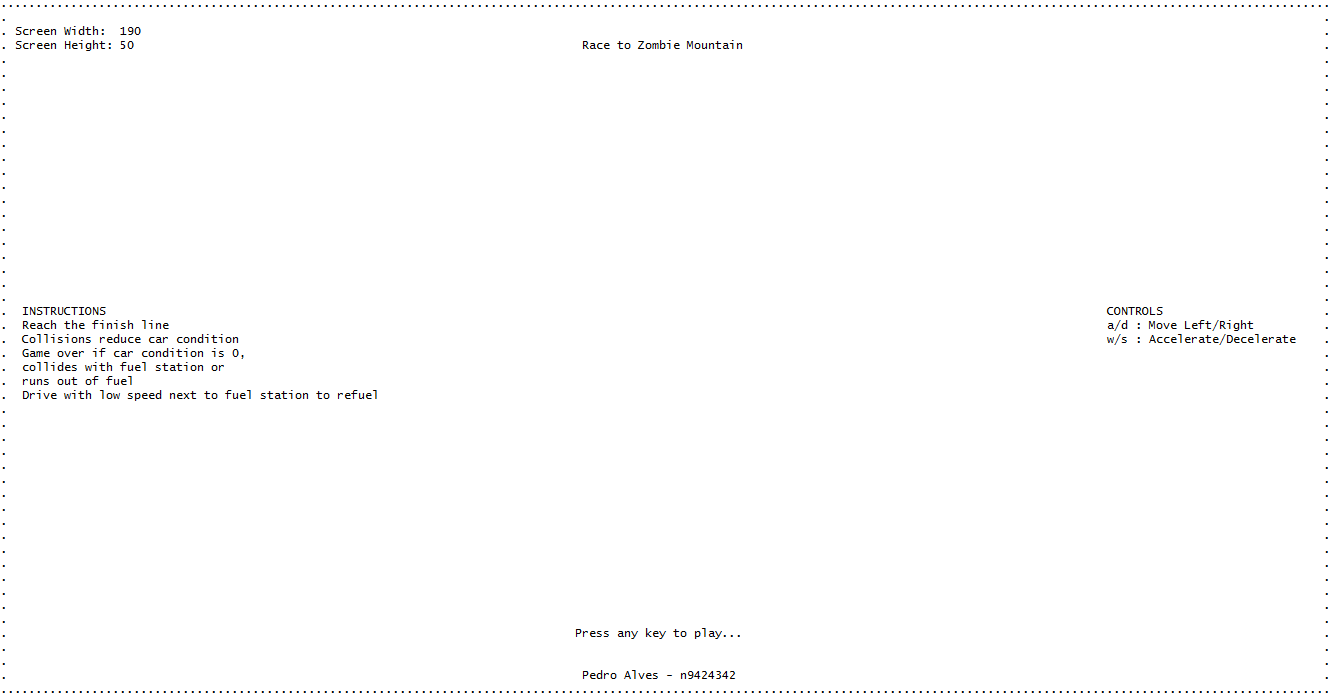
\includegraphics[width=0.77\paperwidth]{images/border_190x50}
	\caption{The border with screen dimensions of 190x50}
	\label{fig:border_190x50} 
	\end{center}
\end{figure}

\clearpage
%----------------------------------------------------------------------------------------
%	DASHBOARD
%----------------------------------------------------------------------------------------
\section{Dashboard}
A sub-window in the terminal which displays data regarding the player's car such as condition, speed and fuel as well as displaying stats on the game itself such as time spent and total distance travelled. 
\newline
Warnings also appear on the dashboard to notify the player that the car is offroad or is refuelling.

\subsection*{Globals}
\begin{lstlisting}[style=CStyle]
	// zombiemountain.h
	int dashboard_x;
\end{lstlisting}
The x-coordinate of the border between the dashboard and the playing area.
\begin{lstlisting}[style=CStyle]
	// obstacles.h
	#define DASHBOARD_SIZE	20
\end{lstlisting}
The width of the dashboard.
\begin{lstlisting}[style=CStyle]
	// zombiemountain.h
	#define DASHBOARD_BORDER_CHAR	47
\end{lstlisting}
The ASCII character that will represent the border that separates the playing area and the dashboard.
\begin{lstlisting}[style=CStyle]
	// zombiemountain.h
	int speed;
\end{lstlisting}
The current speed of the player.
\begin{lstlisting}[style=CStyle]
	// zombiemountain.h
	int fuel;
\end{lstlisting}
The current fuel available to the player.
\begin{lstlisting}[style=CStyle]
	// obstacles.h
	int car_condition;
\end{lstlisting}
The condition of the car as a percentage.
\begin{lstlisting}[style=CStyle]
	// hscore.h
	int score;
\end{lstlisting}
The current score of the player.
\begin{lstlisting}[style=CStyle]
	// zombiemountain.h
	int distance_travelled;
\end{lstlisting}
The distance travelled since the start of the game.
\begin{lstlisting}[style=CStyle]
	// zombiemountain.h
	double game_start_time;
\end{lstlisting}
The time in milliseconds that the game started.
\begin{lstlisting}[style=CStyle]
	// zombiemountain.h
	timer_id refuel_timer;
\end{lstlisting}
A timer that is set when the car starts refuelling.
\newline

\subsection*{Functions}
\begin{lstlisting}[style=CStyle]
	// main.c
	void draw_dashboard();
\end{lstlisting}
Draws a border between the playing area and the dashboard area. Calls \emph{draw\_string()} and \emph{draw\_int()} multiple times to print the relevant globals and their captions.
\newline
If the car is offroad or refuelling, a relevant warning will also be drawn. Additionaly for refuelling, will display how long until it is finished.
\newline
\begin{lstlisting}[style=CStyle]
	// main.c
	bool car_offroad();
\end{lstlisting}
Checks if any portion of the car is outside the road boundaries and return true if so.
\begin{lstlisting}[style=CStyle]
	// main.c
	double refuel_time_left();
\end{lstlisting}
Calculates how much time is left to finish refuelling. This is done by calculating the difference between the current time and the time the \emph{refuel\_timer} is meant to reset, this is then subtracted from \emph{3.0}.
\newline

\subsection*{Testing}
\subsubsection*{Stats are modified with gameplay}
Two screenshots of the same gameplay are taken where the fuel is checked if it is decreased and the time,distance and score are increased.
\begin{figure}[!ht]
	\begin{center}
	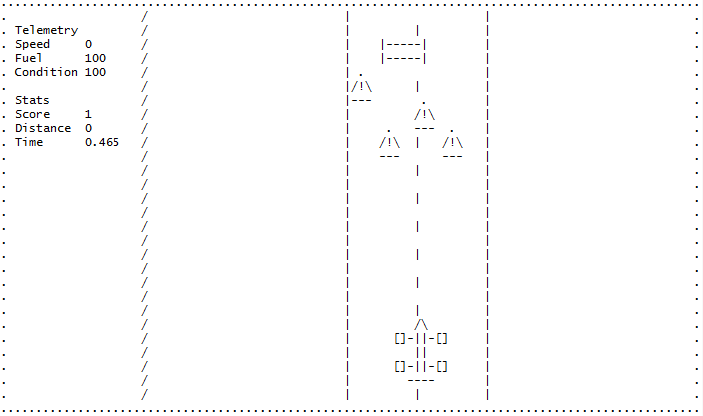
\includegraphics[width=0.75\paperwidth]{images/dashboard_test_statschange}
	\caption{A screenshot of the game as it starts}
	\label{fig:dashboard_test_stats} 
	\end{center}
\end{figure}
\newline
Figure \ref{fig:dashboard_test_stats} shows the dashboard on the left side of the terminal with a border clearly separating it from the playing area. To achieve the second part of the test, the 'w' key was pressed 3 times to test if the speed is increased and the car was moved horizontally where necessary to avoid obstacles. 
\newline
The condition stat will be tested in the \emph{Collision} section and the refuelling warning and timer will be tested in the \emph{Fuel} section.  
\newpage
\begin{figure}[!ht]
	\begin{center}
	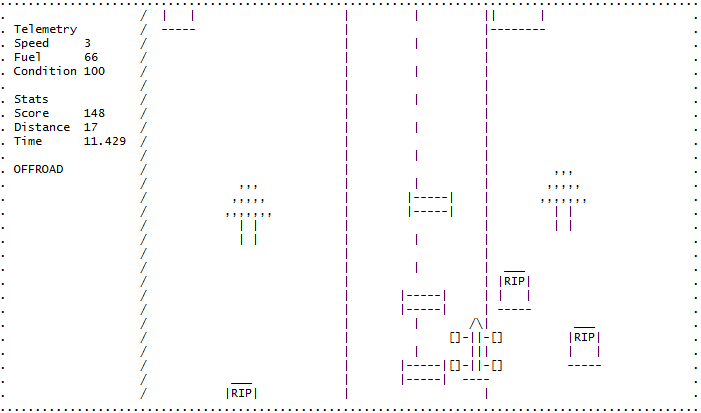
\includegraphics[width=0.75\paperwidth]{images/dashboard_test_statschange2}
	\caption{A screenshot of the same game sessions as the figure above but 11 seconds into gameplay}
	\label{fig:dashboard_test_stats2} 
	\end{center}
\end{figure}
Figures \ref{fig:dashboard_test_stats} and \ref{fig:dashboard_test_stats2} show that the stats are represented in the dashboard and change when supposed to. The \emph{OFFROAD} warning also appears when the car moves beyond the border of the road. 
\newline
Figure \ref{fig:dashboard_test_fuelwarning} shows the low fuel warning appears when fuel falls below 25\%.
\begin{figure}[!ht]
	\begin{center}
	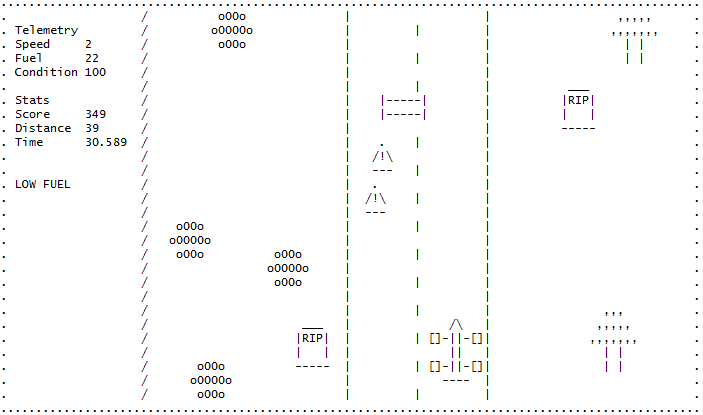
\includegraphics[width=0.667\paperwidth]{images/dashboard_test_fuelwarning}
	\caption{Low Fuel warning appearing when fuel is below 1/4 the maximum}
	\label{fig:dashboard_test_fuelwarning} 
	\end{center}
\end{figure}
\clearpage

%----------------------------------------------------------------------------------------
%	RACE CAR AND HORIZONTAL MOVEMENT
%----------------------------------------------------------------------------------------
\section{Race Car and Horizontal Movement}
The race car is a sprite 8 units wide and 5 units tall. This sprite is always stuck in the same position with the illusion of movement given by the obstacles being moved downwards. The speed at which the obstacles move is proportional to the speed setting.

\subsection*{Globals}
\begin{lstlisting}[style=CStyle]
	// imagemngr.h
	#define PLAYER_WIDTH	8
\end{lstlisting}
The width of the car sprite.
\begin{lstlisting}[style=CStyle]
	// imagemngr.h
	#define PLAYER_HEIGHT	5
\end{lstlisting}
The height of the car sprite
\begin{lstlisting}[style=CStyle]
	// zombiemountain.h
	#define INPUT_MOVE_LEFT		'a'
\end{lstlisting}
The keyboard input that will make the car turn left.
\begin{lstlisting}[style=CStyle]
	// zombiemountain.h
	#define INPUT_MOVE_RIGHT	'd'
\end{lstlisting}
The keyboard input that will make the car turn right
\begin{lstlisting}[style=CStyle]
	// zombiemountain.h
	sprite_id player;
\end{lstlisting}
The car sprite which the player controls.
\newline

\subsection*{Functions}
\begin{lstlisting}[style=CStyle]
	// main.c
	void setup_player_car();
\end{lstlisting}
Place the car sprite in the middle of the road, 2 units above the bottom of the screen. Also sets the car condition to 100\% and fuel to max.
\begin{lstlisting}[style=CStyle]
	// main.c
	void handle_input();
\end{lstlisting}
Get the next character from the input buffer. If it is a valid key, call the specific input handler. 
\begin{lstlisting}[style=CStyle]
	// main.c
	void handle_movement_input(int key);
\end{lstlisting}
Checks if the \emph{key} variable wants the car to turn left or right. Will then check if the car will be in the bounds of the playing area, if it'll collide laterally with any obstacle and if the speed is above zero. If all three checks pass, then the \emph{sprite\_move()} function is called.
\begin{lstlisting}[style=CStyle]
	// main.c
	bool in_bounds(int x, int y)
\end{lstlisting}
Checks if the \emph{(x,y)} coordinate is in bounds of the playing area, returns true if so.
\newline
\newpage

\subsection*{Testing}
\subsubsection*{Car doesn't move when speed is 0}
\begin{figure}[!ht]
	\begin{center}
	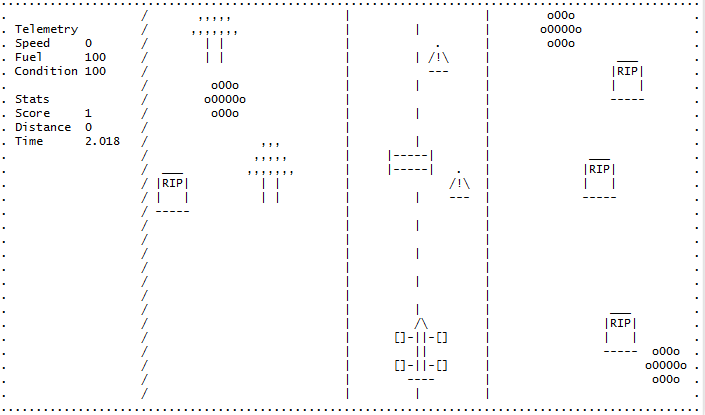
\includegraphics[width=0.667\paperwidth]{images/car_test_nospeed}
	\caption{Car in the middle of the road with speed equal zero}
	\label{fig:car_test_nospeed} 
	\end{center}
\end{figure}
The following inputs were pressed and the result shown in Figure \ref{fig:car_test_nospeed}: "a,d,a,d"
\begin{figure}[!ht]
	\begin{center}
	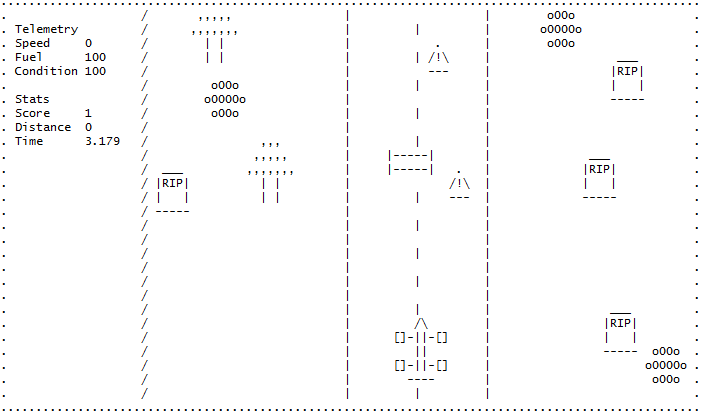
\includegraphics[width=0.667\paperwidth]{images/car_test_nospeed2}
	\caption{Results after attempting to move horizontally with speed equal zero}
	\label{fig:car_test_nospeed2} 
	\end{center}
\end{figure}

\subsubsection*{Car moves left and right}
From the position in Figure \ref{fig:car_test_nospeed2}, the following inputs were pressed "w,a,a,a".
\begin{figure}[!ht]
	\begin{center}
	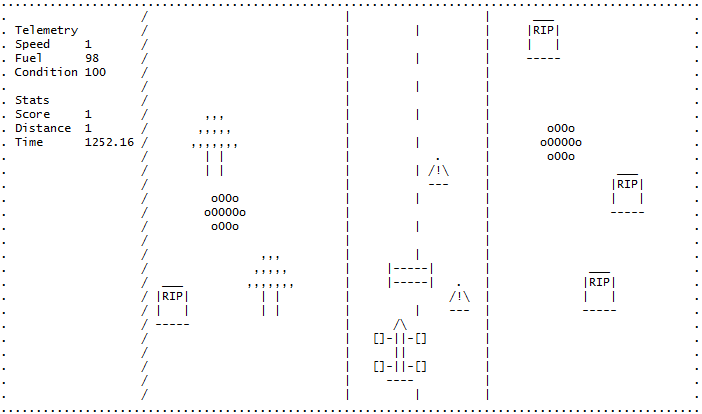
\includegraphics[width=0.667\paperwidth]{images/car_test_moveleft}
	\caption{Moving the car left with speed equal 1}
	\label{fig:car_test_moveleft} 
	\end{center}
\end{figure}
\newline
After the car is reset due to the inetivable collision in Figure \ref{fig:car_test_moveleft}, the following inputs were pressed "w,d,d,d". 
\begin{figure}[!ht]
	\begin{center}
	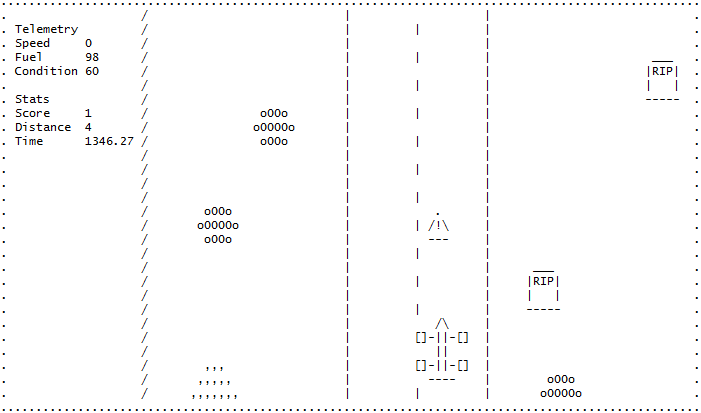
\includegraphics[width=0.667\paperwidth]{images/car_test_moveright}
	\caption{Moving the car right with speed equal 1 (car was stopped to grab screenshot)}
	\label{fig:car_test_moveright} 
	\end{center}
\end{figure}
\newpage

\subsubsection*{Car stays in bounds}
The car was moved to both extremes of the playing area with the lateral movement input held down. Figure \ref{fig:car_test_rightborder} shows the result of holding down 'd' and Figure \ref{fig:car_test_leftborder} shows the result of holding down 'a'.
\begin{figure}[!ht]
	\begin{center}
	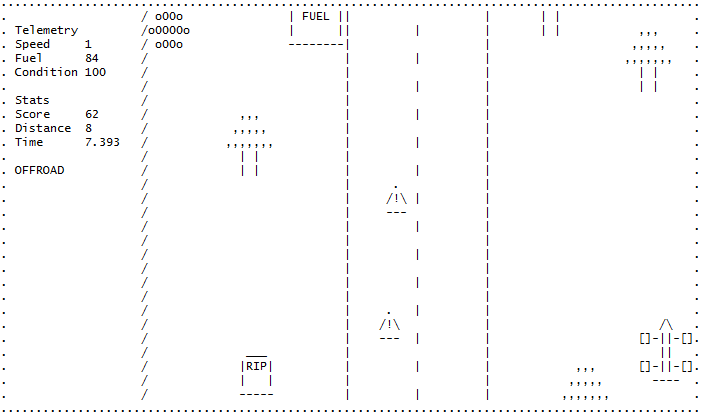
\includegraphics[width=0.667\paperwidth]{images/car_test_rightborder}
	\caption{Result of holding down 'd' when next to the right border}
	\label{fig:car_test_rightborder} 
	\end{center}
\end{figure}
\begin{figure}[!ht]
	\begin{center}
	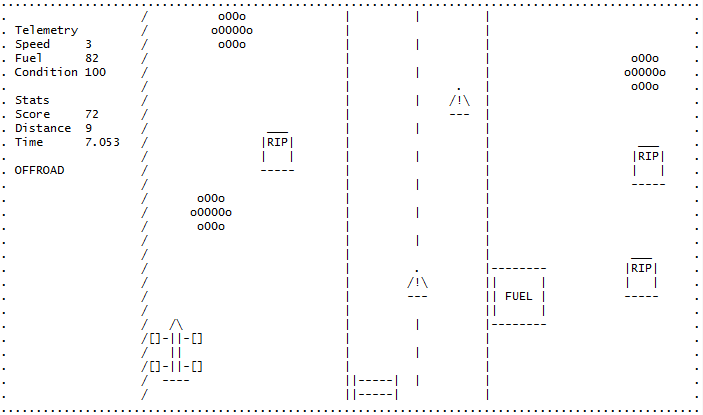
\includegraphics[width=0.667\paperwidth]{images/car_test_leftborder}
	\caption{Result of holding down 'a' when next to the left border}
	\label{fig:car_test_leftborder} 
	\end{center}
\end{figure}

\clearpage

%----------------------------------------------------------------------------------------
%	ACCELERATION AND SPEED
%----------------------------------------------------------------------------------------
\section{Acceleration and Speed}
The car can accelerates and decelerates with the 'w' and 's' keys. The speed can never go negative or higher than 10. When the car is offroad (indicated by the \emph{OFFROAD} warning in the dashboard) the speed is limited to a maximum of 3.

\subsection*{Globals}
\begin{lstlisting}[style=CStyle]
	// zombiemountain.h
	#define INPUT_ACCELERATE	'w'	
\end{lstlisting}
The character input to accelerate the car.
\begin{lstlisting}[style=CStyle]
	// zombiemountain.h
	#define INPUT_DECELERATE	's'
\end{lstlisting}
The character input to decelerate the car.
\begin{lstlisting}[style=CStyle]
	// zombiemountain.h
	#define MAX_SPEED			10
\end{lstlisting}
The maximum speed the car can reach.
\begin{lstlisting}[style=CStyle]
	// zombiemountain.h
	#define MAX_SPEED_OFFROAD	3
\end{lstlisting}
The maximum speed the car can reach while offroad.
\begin{lstlisting}[style=CStyle]
	// zombiemountain.h
	#define SPEED_INTERVAL	87
\end{lstlisting}
Used to set the reset time for \emph{speed\_timer}.
\begin{lstlisting}[style=CStyle]
	// zombiemountain.h
	#define LOOP_INTERVAL	17
\end{lstlisting}
Used with \emph{SPEED\_INTERVAL} and \emph{speed\_timer} to decide when to increment \emph{speed\_ctr}.
\begin{lstlisting}[style=CStyle]
	// zombiemountain.h
	int speed;
\end{lstlisting}
The speed of the player, this affects how fast the obstacles scroll down.
\begin{lstlisting}[style=CStyle]
	// zombiemountain.h
	int speed_ctr;
\end{lstlisting}
Is compared with the current speed to decide when to update the main game logic (increasing distance, making obstacles scroll, etc.).
\begin{lstlisting}[style=CStyle]
	// zombiemountain.h
	timer_id speed_timer;
\end{lstlisting}
This timer controls when \emph{speed\_ctr} is increased.
\newpage

\subsection*{Functions}
\begin{lstlisting}[style=CStyle]
	// main.c
	void setup_player_car();
\end{lstlisting}
Place the car sprite in the middle of the road, 2 units above the bottom of the screen. Also sets the car condition to 100\% and fuel to max.

\clearpage

%----------------------------------------------------------------------------------------
%	SCENERY AND OBSTACLES
%----------------------------------------------------------------------------------------
\section{Scenery and Obstacles}

\clearpage

%----------------------------------------------------------------------------------------
%	FUEL DEPOT
%----------------------------------------------------------------------------------------
\section{Fuel Depot}

\clearpage

%----------------------------------------------------------------------------------------
%	FUEL
%----------------------------------------------------------------------------------------
\section{Fuel}

\clearpage


%----------------------------------------------------------------------------------------
%	DISTANCE TRAVELLED
%----------------------------------------------------------------------------------------
\section{Distance Travelled}

\clearpage


%----------------------------------------------------------------------------------------
%	COLLISION
%----------------------------------------------------------------------------------------
\section{Collision}

\clearpage


%----------------------------------------------------------------------------------------
%	GAME OVER DIALOGUE
%----------------------------------------------------------------------------------------
\section{Game Over Dialogue}

\clearpage

%----------------------------------------------------------------------------------------
%	PARTB
%----------------------------------------------------------------------------------------
\section{Part B - Highscore Screen}

\clearpage



%----------------------------------------------------------------------------------------
%	REFERENCES
%----------------------------------------------------------------------------------------
\section{References}

\clearpage

\end{document}
